\documentclass[10pt, a4]{article}

\usepackage[T1]{fontenc}
\usepackage{cogsci}
\usepackage{pslatex}
\usepackage{gb4e}
\noautomath

\usepackage[round]{natbib}
\usepackage{graphicx}

\usepackage[english]{babel}

\usepackage{blindtext}

\graphicspath{{img/}}

\title{Do adults behave like children when under pressure?}

\author{{\large \bf Samuel Giacomelli (S.Giacomelli@student.rug.nl)} \\
University of Groningen}

\begin{document}

\maketitle

\begin{abstract}
    Do adults behave like children when under pressure? If children perform
    differently because they have more limited cognitive resources, like working
    memory, if you load adults working memory can you then get them to show childlike
    behavior/interpretations?   
\end{abstract}

\section{Introduction}
\section{Symmetrical Response and Logical Reading}

\section{Universal quantification}
Investigate on adult tendency to commit universal quantification when their cognitive resources are limited.\\
\textit{The present study aims at examining this hypothesis}.\\
\\
Symmetrical response (SR) and Logical reading (LG) in children and adults do to low level of \textit{COGNITIVE CONTROL}.
Multiple numbers (>= 6) of extra objects almost perfect LG (\cite{sugisaki2001quantification}).\\
Desired number of extra object should be the one that is capable to elicit both LG and SR responses.\\
Ability to flexibly switch perspective, children are inflexible (\cite{piaget1954language}).\\
Children between 4 and 5 yo as in (\cite{minai2012hinders}). Because they're able to provide both SR and LG responses\\
One group of adults 20-30.\\
\textit{Question-answer Requirement} -> sentences are interpreted as answers to particular questions. Maybe
under pressure the participant tend to find easier question, leading to commit errors and universal quantification.\\

\section{Present Study}
Truth Value Judgment (TVJ) task (\cite{crain2000investigations})
Use both extra object and extra subject picture.\\

For this experiment we will use materials very similar to the one used in \cite{minai2012hinders},
with the difference that in addition to under exhaustive scenes, in which objects are more than subjects,
we will provide also over exhaustive ones (i.e. images in which subjects are greater in number than objects).
Another important change to the original images will be done and it will consist in moving
the extra objects, or the extra subjects, respectively, in all the four lattices in which
the image is divided. This hasn't been done in the work of \cite{minai2012hinders} and it could
have led to a lack of processing of the image presented.


\section{Method}
\subsection{Participants}
Our participants will be divided in two groups. The first one will be the \textit{CONTROL} and is going to be
composed by around 40 english acquiring children between 4 and 5 years old, while the \textit{TARGET} group will consist
of at least 40 english native speakers adults between 20-40\footnote{Subjects in this age span should have completely developed
their linguistic and cognitive skills} years old. Both the \textit{CONTROL} and the \textit{TARGET} group will be composed in equal
parts by males and females in order to provide more consistent and reliable data for the analysis.
The participants of the CONTROL group will have to complete just the \textit{TVJ} task to determine the baseline of the childlike behavior,
while the one composing the TARGET group will have to complete both the \textit{SDR} and the \textit{TVJ} task simultaneously.

\subsection{Procedure}
\subsubsection{Children}
Children will be presented a picture in the top centre of a display followed after 2500ms by a spoken sentence,
in the exact moment that they start hearing the sentence they have to move the mouse toward the answer they think it
is correct, in our case the possible answers are "YES/NO" and are presented in two boxes on the left and on the
right of the picture. If the children are too slow in the beginning they will be asked to begin moving the mouse earlier.
In order to display the picture and start the single step of the task children will have to click on a start button,
the picture will be presented and then in the same moment when they start hearing the sentence the two boxes containing "YES" and "NO"
will appear on the screen.
Knowing that this can be demanding for the children we take in account the possibility for them to take a break during
the execution of the experiment (approximately in the middle).

\subsubsection{Adults}
For adults the \textit{TVJ} task will be presented in the same way, with the only difference that they won't be able to take
a break during the experiment. Furthermore they will be asked to go through a Span Digit Recall (\textit{SDR}) tasks while
completing the first one. This task consists in displaying on the screen a digit every three steps of the \textit{TVJ} task
and asking at the end of the experiment to recall the digits in the correct sequence of presentation. When adults press the start button
for the first time a digit will appear on the screen and will stay there for 1 second. After this period of time the first part of the \textit{TVJ}
task will begin and after three steps this procedure will be repeated and another digit will be shown on the screen.
In this way in the end they will have to remember a total of six digits which in accord of the findings of \cite{taub1972comparison}
is a little bit below the maximum number of digits that an average 30yo adult can remember. The way chosen to propose the \textit{SDR} task is specifically
thought to progressively increase the load on the working memory of the subjects, letting them with less available cognitive resources
to process the response to the \textit{TVJ} task's questions and trying to elicit in them a childlike behavior.


\subsection{Materials}
\subsubsection{Sentences}
As this study is partially inspired by the work of \cite{minai2012hinders}, the stimuli used for the \textit{TVJ} task are the
english translations of the ones presented in their paper, with the only difference that is necessary to add a
\textit{filler item} in order to have an even number of stimuli, which are necessary to divide the task in two blocks.
The stimuli sentences are therefore 18 and are divided in three groups, respectively: 8 target sentences, 8 filler sentences
and 2 warm-up sentences. Below we report an example of a target sentence (\ref{sample_target_sentence}), in (Appendix I) it's possible
to find the complete set of stimuli sentences. All the sentences will be spoken by both a male and a female english native speaker and
recorded in order to be presented to the participants in form of an audio track.

\begin{exe}
    \ex  Every turtle is holding an umbrella. \label{sample_target_sentence}
\end{exe}

Differently from \cite{minai2012hinders} we associated to the target sentences both the under and over-exhaustive scenes. This means
that we have 2 showable stimuli for each sentence. Participants are presented in the same proportion under and over-exhaustive ones,
respectively four for each type, but they are never presented the same sentence with the two different images that describe it, in order to avoid priming.
In addition another change will be done on the images used in the above cited study that consist in moving the extra object in different positions
of the image. Since in the original paper they were always in the bottom right lattice, we think that this disposition made the children focus their
attention always on a minimal part of the image and in particular on the extra objects. Below (Figure \ref{img-target-sample}) we report an example of the images that
will be used in our research.

\begin{figure} [!ht]
    \begin{minipage}{0.48\textwidth}
      a.
      \centering
      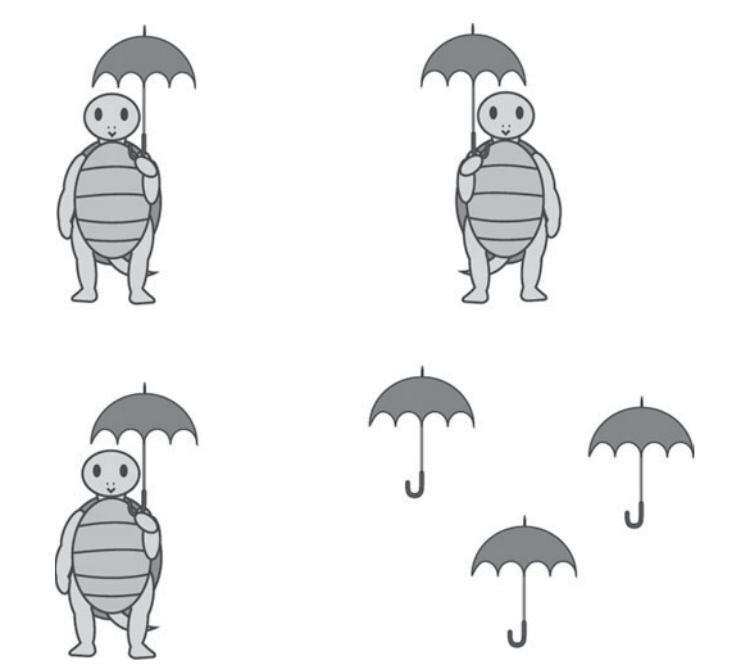
\includegraphics[width=.7\linewidth]{proj_prop_turtles_under_exhaustive.png}
      \label{img-target-under-exhaustive}    
    \end{minipage}
    \begin {minipage}{0.48\textwidth}
      b.
      \centering
      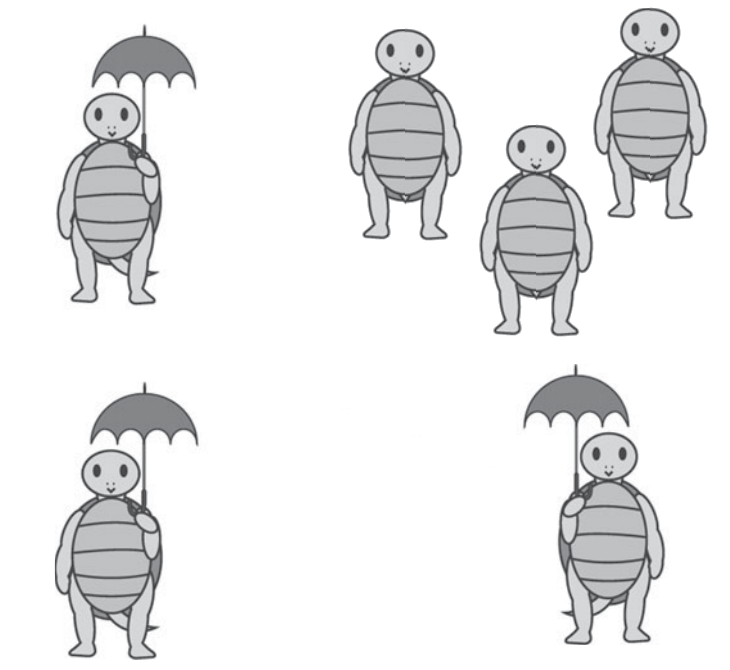
\includegraphics[width=.7\linewidth]{proj_prop_turtles_over_exhaustive.png}
      \label{img-target-over-exhaustive}
    \end{minipage}
    \caption{Example of images used in the experiment. Picture a. shows the under exhaustive case, while picture b. the over exhaustive one}
    \label{img-target-sample}
\end{figure}


\subsection{Digits' sequences}
The stimulus sets consisted in sequences of six digits each (one every three steps of the \textit{TVJ} task), each of them from 1 to 9 without
repetition within the same sequence. Furthermore, according to the work of \cite{taub1972comparison} one more restriction will be applied on the sequences,
which consists in not presenting adjacent pairs of digits in the correct counting order (neither increasing or decreasing).

\section{Results}
\blindtext

\section{Discussion}
\blindtext


\bibliographystyle{plainnat}

\setlength{\bibhang}{.125in}
\setlength{\bibindent}{-\bibhang}

\vfill
\pagebreak

\bibliography{giacomelli_samuel_pp}

\appendix
\section{Appendix I} \label{appendix_I_sentences}


\end{document}
